\documentclass[12pt]{ociamthesis}
\setlength{\topmargin}{0.0in}
\setlength{\oddsidemargin}{0.33in}
\setlength{\textheight}{9.0in}
\setlength{\textwidth}{6.0in}
\renewcommand{\baselinestretch}{1.25}
%load any additional packages
\usepackage{amssymb}
\usepackage{hyperref}
% \usepackage[utf8]{inputenc}
% \usepackage[T1]{fontenc}
\usepackage{float}
\usepackage{enumitem}
\usepackage{amsmath}
\usepackage{amssymb}
\usepackage{tikz}
\usetikzlibrary{decorations.pathreplacing}
\usepackage{amsfonts}
\usepackage{graphicx}
\usepackage{subcaption}
\usepackage{caption}
\newcommand{\dv}[2]{\frac{\mathrm{d} #1}{\mathrm{d} #2}}
\usepackage{caption}
\captionsetup[figure]{font=small} 
% \captionsetup[table]{font=small}
\usepackage[capitalize,nameinlink]{cleveref}
\usepackage{mathtools}
\newcommand{\defeq}{\vcentcolon=}
\newcommand{\eqdef}{=\vcentcolon}
%\usepackage{amssymb,amsmath,epsfig,html}

\title{Efficient Algorithms for Infinite-Dimensional Spectral Computations}   %note \\[1ex] is a line break in the title
\author{Margaret McCarthy}             %your name
\college{Christ Church College}  %your college
%\renewcommand{\submittedtext}{change the default text here if needed}
%\degree{M. Sc. in Mathematical Modelling and Scientific Computing}     %the degree
%\degreedate{Trinity 2026}         %the degree date

%\renewcommand{\submittedtext}{Dissertation submitted in partial fulfilment of the requirements for the degree of}
\degree{M.Sc.\ in Mathematical Modelling and Scientific Computing}
\degreedate{Trinity Term 2026}

\renewcommand{\baselinestretch}{1.25}
\begin{document}
\include{macpap2}

\setcounter{secnumdepth}{3}
\setcounter{tocdepth}{2}

\maketitle
\begin{acknowledgements} 

I would like to thank my supervisors, Patrick Farrell and Umberto Zerbinati, for their continued guidance and support. 
This dissertation has introduced me to a whole world of interesting research questions that I cannot wait to explore further.

I am also grateful to both Matthew Colbrook and Daniele Boffi for the valuable discussions I had with them regarding this work.

Finally, I would like to thank my family, friends, and partner, Ben, who have supported me in an uncountably infinite number of ways. 

\end{acknowledgements}

\begin{abstract}

Fill later
  
\end{abstract}


\begin{romanpages}
\tableofcontents
\listoffigures
\listoftables
\end{romanpages}

\chapter{Introduction}

% The importance of spectra cannot be overstated, and the study of spectra has a long and rich history in mathematics.

With at least twenty Nobel Prizes in Physics coming from phenomena associated with eigenvalues, and thus with spectra, it is hard to overstate the importance of spectra in applied mathematics (Nick's essay). Indeed, spectra play a major role in numerous fields, such as acoustics, chemical analysis, dynamical systems, fluid mechanics, quantum mechanics, and partial differential equations (PDEs) \footnote{For an overview of the history and applications of eigenvalue problems, which are a subset of spectral problems, see the introduction of (Nicks text) and the references therein.}. For example, the black `Fraunhofer lines' that appear in spectroscopic images of the sun's light, such as in Figure ?, correspond to the differences of eigenvalues of the Schrödinger operator for atoms such as H, Fe, Ca, Na, and Mg (Nick). Spectroscopic measurements such as these allowed for the measurement of redshifts of distant galaxies, leading to the discovery of the expanding universe (Nick).
\begin{figure}[ht]
    \centering
    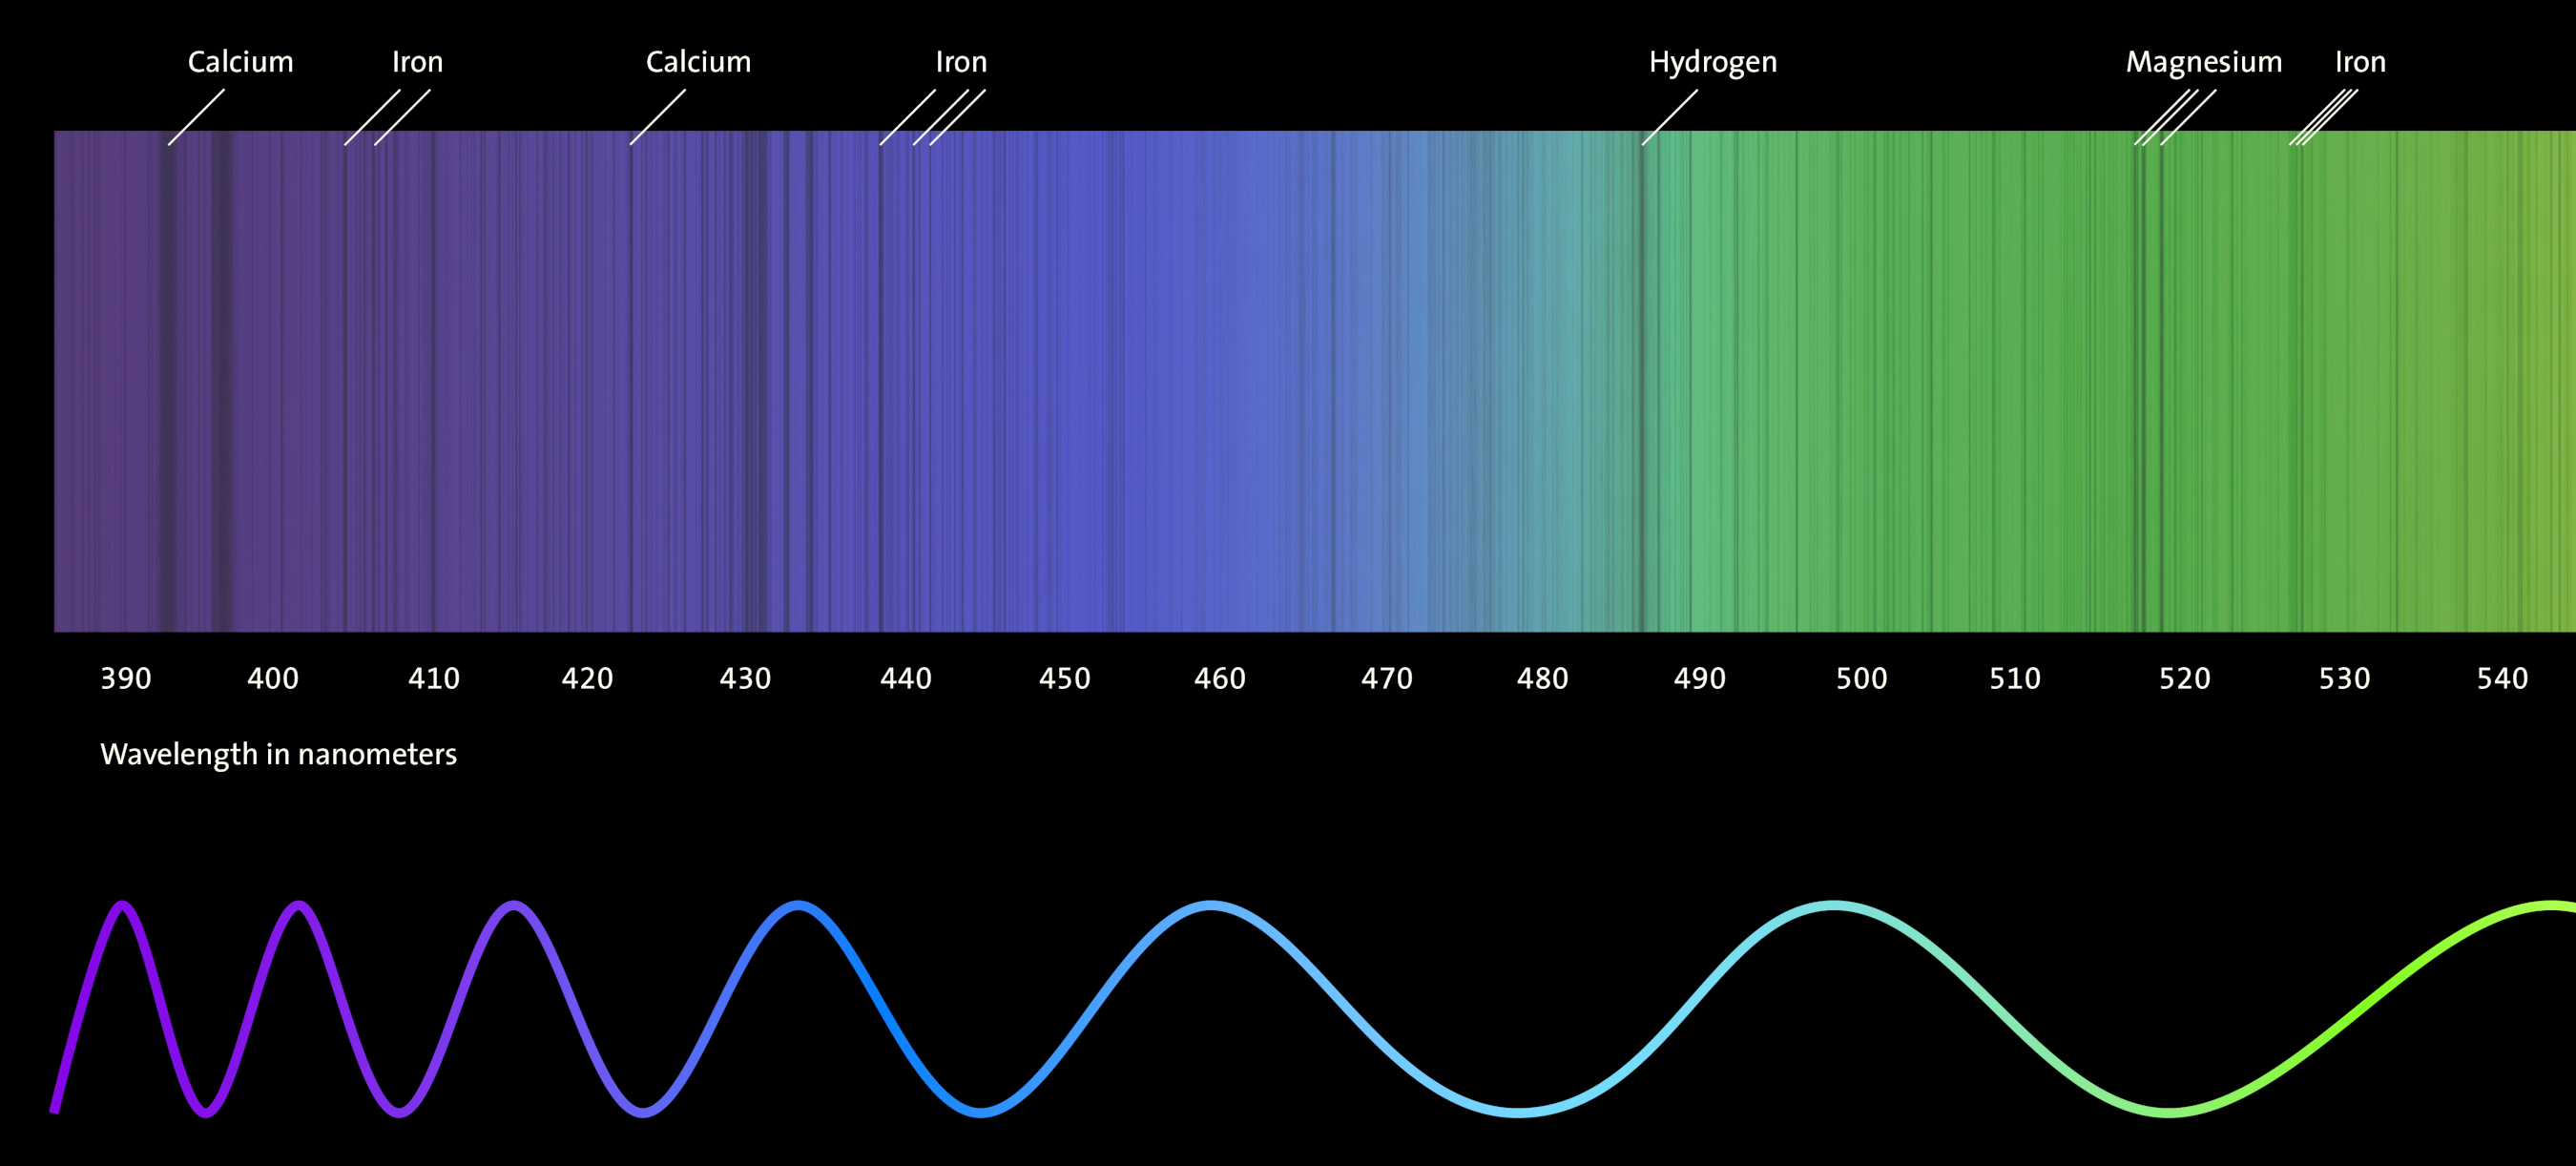
\includegraphics[width=0.48\linewidth]{images/griff_2.jpg}
    \hfill
    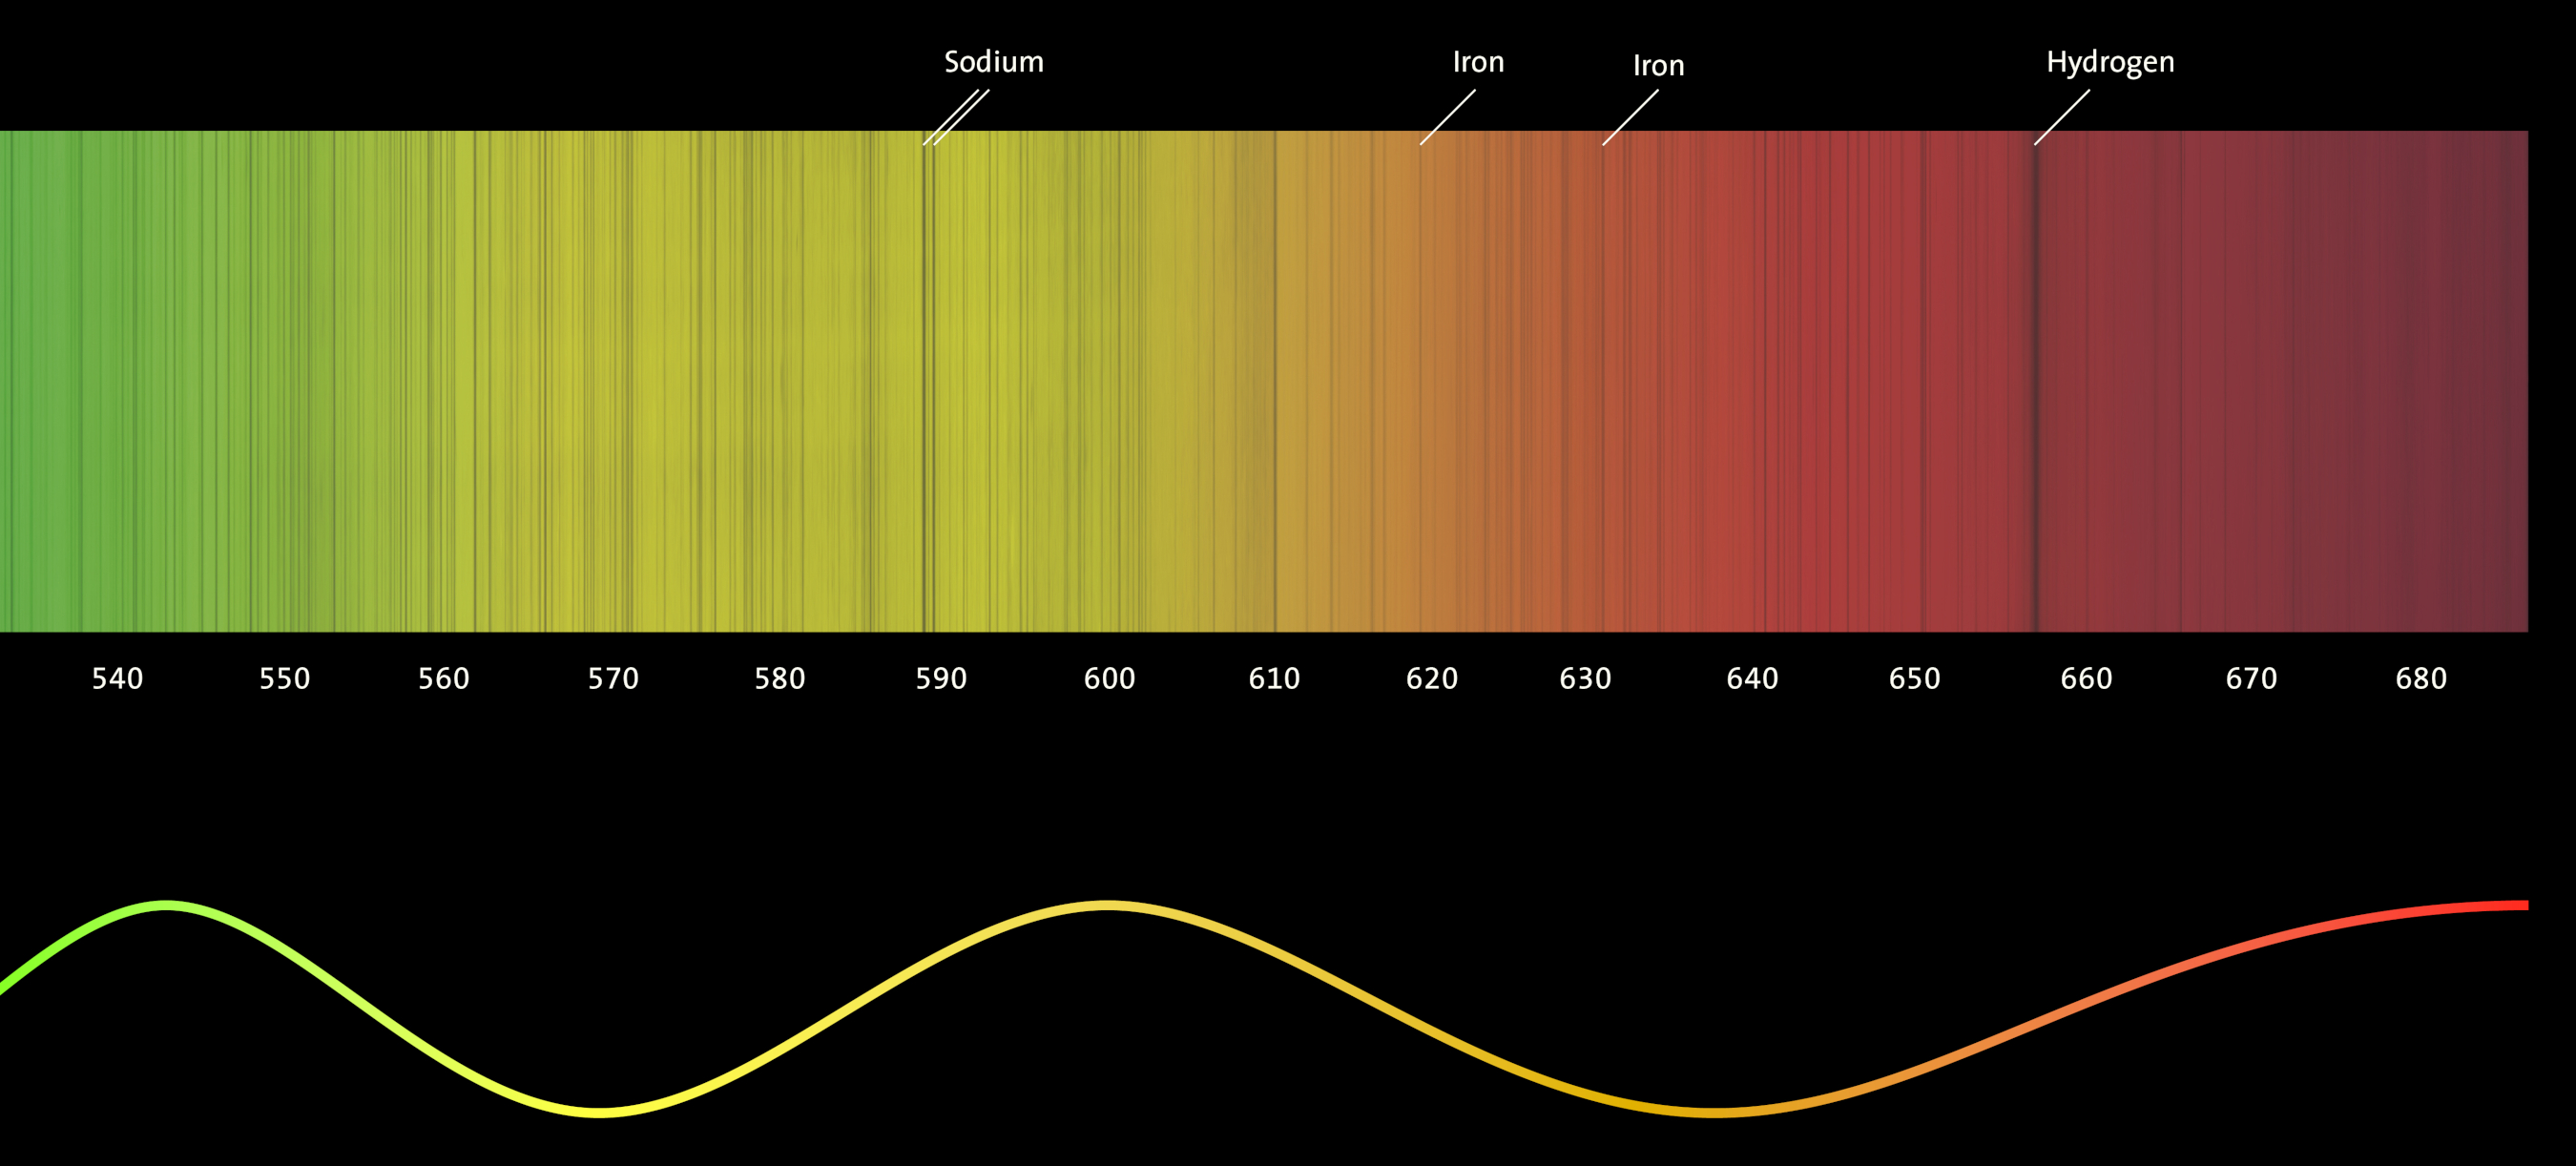
\includegraphics[width=0.48\linewidth]{images/griffith_lines.jpg}
    \caption{Spectroscopic images of the sun's light, courtesy of the Griffith Observatory.}
    \label{fig:spectroscopic-images}
\end{figure}

Although the importance of spectra is beyond question, their reliable computation is another matter (preface). In finite dimensions, we compute matrices, whose spectrum is the set of their eigenvalues. In particular, if $B \in \mathbb{C}^{nxn}$ then its spectrum is the following set of points:
\begin{equation} \label{matrix spec}
    \operatorname{Sp}(B) = \{z \in \mathbb{C}: \det (B-zI) = 0 \} = \{z \in \mathbb{C}: (B-zI)^{-1} \text{ does not exist} \},
\end{equation}
where $I$ denotes the identity matrix. 
% One might be tempted to think that this is a straightforward problem. However, as we will see, even for non-normal matrices, computed eigenvalues may be unreliable. 
In infinite dimensions, we consider a linear operator $A$ on a Hilbert space $H,$ whose spectrum is defined by the following set:
\begin{equation} \label{SpA}
    \operatorname{Sp}(A) = \{z \in \mathbb{C}: (A-zI)^{-1} \text{ does not exist as a bounded operator on } H \},
\end{equation}
where $I$ denotes the identity operator. The spectrum of a linear operator includes the set of eigenvalues of $A,$ but is generally much richer (Matt). This follows from the fact that in infinite dimensions there are more ways for $A-zI$ to fail to have a bounded inverse. As a result, new phenomena are present in the spectra of linear operators that make them much harder to reliably compute. To see this, consider the right-shift operator, 
\begin{equation}\label{right shift}
    A(x_1, x_2, \dots) = (0, x_1, x_2, \dots),
\end{equation}
that acts on a square-summable\footnote{Claiming that a sequence is `square-summable' is claiming that the sequence is in $l^2.$ The $l^2$ space consists of the space of sequences $(x_n)_{n\in \mathbb{N}}$  that satisfy $\sum_n x_n^2 < \infty.$} sequence of points, $(x_n)_{n\in \mathbb{N}}.$  This operator's spectrum is equal to the unit disc, but it has no eigenvalues\footnote{For more information on this example, see Appendix ?}.

The standard approach for computing the spectra of an infinite-dimensional operator is often refered to as the \textit{discretize-then-solve} approach. This approach consists of discretizing the operator with a finite-dimensional matrix, computing the spectrum of the discretized operator, and hoping that the spectrum of the discretized operator approaches the spectrum of the infinite-dimensional operator as the size of the discretization increases. Despite being a successful approach for many problems, it is fraught with difficulties. If the problem is not discretized very carefully, \textit{spectral pollution} can occur, where the discretized operator has eigenvalues that converge to something not in the spectrum of the infinite-dimensional operator (Patrick). Furthermore, the approach can suffer from \textit{spectral invisibility}, where discretizing the operator causes us to miss parts of the spectrum, even as the size of the discretization increases. Even if our discretization manages to avoid both spectral pollution and spectral invisibility, there remains a far more catastrophic limitation of the discretize-then-solve approach. In particular, since the spectra of infinite-dimensional operators may include more than just eigenvalues of finite multiplicity, there may be parts of the spectrum that we can never capture with the finite, discrete set of eigenvalues that results from discretization. 

These major pitfalls of the discretize-then-solve approach motivate the development of alternative methods for computing the spectra of infinite-dimensional operators. This challenge has been taken up by Matthew Colbrook at Cambridge. In recent work, Colbrook has proposed a new algorithm for computing the spectra of infinite-dimensional operators. Under certain conditions on the operator, this method yields a convergent approximation of the spectrum that captures the continuous components of the spectrum and does not suffer from spectral pollution or spectral invisibility. 
\begin{itemize}
    \item Quick overview of the algorithm
    \item Issues with it
    \item Our ideas 
\end{itemize}




% For example, if the range of $(A-zI)$ is not all of $H,$ $z \in \operatorname{Sp}(A)$ even if $z$ is not an eigenvalue of $A.$

% As a result, the study of spectra has a long and rich history. 
% Long before the development of modern spectral theory, humans observed that a stretched string does not produce just one sound, but a collection of related sounds (Matts forward). From these observations came the central thought that complicated motion may be understood through the combination of simpler oscillatory components. 
% Spectral theory in the modern sense, is often traced back to Fourier's solution of the the heat equation with series expansions, along with Euler and Lagrange'sstudy of eigenvectors in relation to rigid body motion (Matt, Preface). The field continued to be developed in the 19th century with contributions from scientists such as Cauchy, Cayley, Hermite, Liouville, Poincaré, Poisson, Rayleigh, Schwarz, Sturm, and Sylvestor (preface). In the 20th century, Hilbert's use of infinite matrices to study the eigenvalues of integral operators shaped much of the infinite-dimensional spectral theory considered today. Weyl extended the thoery to singular second-order ordinary differential equations (ODEs), von Neumann pioneered spectral theory for unbounded self-adjoint operators, and Riesz and Stone ...? 


\section{Motivations and  Project Goals}

\section{Main Contributions}
The examiners have suggested that a ``main contributions'' section in the introduction is really useful, so please ensure you have such a section! You can use this to explain what you believe are the main results of your work. If any of what you have done is novel, it can be helpful to highlight that here. If you have worked on an industrial project you could state how and why your results are useful to your industrial partner.

\section{Structure of the Dissertation}
It is common, although not compulsory, to end the introduction with a brief section explaining the structure of the dissertation. Often this goes along the lines of:
The remainder of the dissertation is structured as follows. In Chapter 2 we discuss blah blah. In Chapter 3 we blah blah. Finally in Chapter 4 we summarise the work we have done and suggest some areas for future research.

\section{Code Availability}
Here you may have a link to your GitHub repository (recommended but not mandatory). You can also make clear whether you have written code from scratch, or based it on other code, or had help from ChatGPT.


\chapter{Background}

\section{A Quick Introduction to Spectra and Pseudospectra}


\section{Dangerous Pitfalls of Using the Finite Element Method for Computing Spectra}
\subsection{An Example of Spectral Pollution: The Maxwell Eigenproblem}

\section{Matthew Colbrook's Algorithm for Computing Spectra}
\subsection{Application to the Maxwell Eigenproblem}

\section{The Dual-Weighted Residual Method for Eigenproblems}
\subsection{Application to the Maxwell Eigenproblem}

\chapter{Methodology}

\section{The Inner Loop: Pairing Colbrook's Algorithm with Adaptivity}

\section{The Outer Loop: Adaptively Refining the Complex Plane in Colbrook's Algorithm}

\chapter{Results}


\chapter{Conclusions and Future Work}


In this dissertation, we developed a methodology for accurate and efficient infinite-dimensional pseudospectral computations. To do so, we first explored Colbrook's algorithm for infinite-dimensional pseudospectral computations. This approach characterizes the pseudospectrum of a closed and densely defined linear operator $A$ using the smallest spectral values of the folded operators $(A-zI)^*(A-zI)$ and $(A-zI)(A-zI)^*.$ In doing so, it avoids discretizing the operator $A$ directly. Instead, it discretizes the auxiliary eigenproblems that characterize the smallest spectral values of the folded operators. This delayed discretization underpins the success of Colbrook's algorithm, which avoids the common pitfalls of the standard discretize-then-solve approach.

After exploring the abstract formulation of Colbrook's algorithm, we reformulated it for the setting in which the auxiliary eigenproblems are discretized with the finite element method. We then demonstrated the success of this approach by comparing it to the standard discretize-then-solve approach for the Maxwell eigenproblem. 

% by comparing its performance to the performance of the discretize-then-solve approach when applied to the Maxwell eigenproblem.

% by applying both to the Maxwell eigenproblem. 

% This approach avoids the common pitfalls of the standard discretize-then-solve approach. To see this, we compared the perfromance of Colbrook's algorithm to the performance of the discretize-then-solve approach when both were applied to the Maxwell eigenproblem. 

These initial experiments revealed that, although the finite element realization of Colbrook's algorithm avoids the pitfalls of the discretize-then-solve approach, its accuracy is limited by the resolution of the underlying auxiliary eigenproblems. 



To address this limitation, we devised an adaptive mesh refinement technique that uses DWR estimates for the auxiliary eigenvalue error to improve the accuracy of our finite element realization of Colbrook's algorithm. This technique refines the finite element mesh in regions where the error estimate is large. It also uses the DWR estimates to correct Colbrook's pseudospectral computations. By applying this approach to the Maxwell eigenproblem, we showed that these two uses of the DWR method can improve both the accuracy and efficiency of Colbrook's approach.

% methodology for pairing the Dual-Weighted Residual (DWR) method for symmetric eigenproblems with our finite element realization of Colbrook's algorithm. Using DWR eigenvalue error estimates, we formulated an adaptive mesh refinement technique that refines the computational mesh in regions where the auxiliary eigenvalue error is large. We also used these error estimates to correct the error in Colbrook's pseudospectral computations. By applying this approach to the Maxwell eigenproblem, we showed that these two applications of the DWR error estimate can improve both the accuracy and efficiency of Colbrook's approach.

Motivated by these results, we developed a methodology for coupling adaptive refinement of the auxiliary eigenproblems with adaptive refinement of the test points used in Colbrook's algorithm. To do so, we first used the DWR eigenvalue error estimate to derive an error estimate for Colbrook's pseudospectral computations. This estimate was used to formulate stopping criteria for our adaptive mesh refinement technique based on the desired accuracy of Colbrook's pseudospectral computations.

We then developed a method for adaptively selecting the test points in Colbrook's algorithm. We took these test points to be the barycentres of a triangulation of the complex plane. For each triangle, we formulated criteria for deciding whether the triangle lies inside or outside the desired $\epsilon$-pseudospectrum, or whether the triangle should be further refined. These classification criteria depend on both the diameter of the triangle and the DWR error estimate for Colbrook's pseudospectral computations. We therefore chose the stopping criterion for each adaptive eigensolve based on the diameter of the corresponding triangle. In this way, our methodology avoids solving the auxiliary eigenproblems to a greater accuracy than what is warranted by the current resolution of the complex plane. 

% Accordingly, these criteria gave rise to a natural coupling of the accuracy of the adaptive eigensolves with the adaptive selection of test points in the complex plane. By choosing the stopping criterion for each adaptive eigensolve based on the diameter of the corresponding triangle in the complex plane, we were able to avoid solving the auxiliary eigenproblems to a greater accuracy than what is warranted by the current resolution of the complex plane. 

% Since the classification criteria depend on both the diameter of each triangle and the associated DWR error estimate, we chose the stopping criterion for each adaptive eigensolve based on the diameter of the corresponding triangle. In this way, our methodology avoids solving the auxiliary eigenproblems to a greater accuracy than what is warranted by the current resolution of the complex plane. 

The success of this coupling was demonstrated through its application to a one-dimensional Dirac-type operator and to the Maxwell operator. In both cases, our methodology focused the computational effort near the pseudospectral contour of interest. 

 In future work,  we would like to apply our current methodology to non-normal operators with more complicated pseudospectra. One example is the advection-diffusion operator explored in \cite{Nick}. To further increase the efficiency of our methodology, we would also like to investigate the use of multilevel methods for exploiting the hierarchy of meshes created by our adaptive mesh refinement technique. 
 
 We would also like to relax some of the underlying assumptions of our methodology so that it can be applied to a broader class of operators. In particular, we would like to extend the DWR method to estimate the error in computing general spectral values. We would also like to extend our finite element formulation of Colbrook's algorithm so that it can accommodate a wider range of operators. 

 % to more operators. In particular, we would like to consider
 
 % like to relax some of the assumptions underlying the current methodology so that it can be applied more broadly. To do so, we would like to extend the DWR method to estimate the error in computing general spectral values. We would also like to extend our finite element formulation of Colbrook's algorithm to handle a broader class of operators. ADD MULTILEVEL
 
 % we would like to be able to apply our approach to the standard poisson problem on a nonconvex domain.
 % WHAT OPERATORS?

 Ultimately, the results of this dissertation demonstrate the potential of pairing adaptivity with Colbrook's algorithm for computing the pseudospectra of infinite-dimensional operators. We hope that the ideas presented here provide a foundation for further work toward accurate and efficient solvers for computing the pseudospectra of a broad class of operators.

% Despite the desire for more analytical and numerical work, the results of this thesis demonstrate the potential of pairing adaptivity with Colbrook's methodology for pseudospectral computations. Going forward, we hope to extend these ideas to further develop accurate and efficient solvers for computing the pseudospectra of a broad class of operators.



% here can be extended toward an efficient framework for accurately computing the pseudospectra of a broad class of operators.

% look forward to extending the current results to the development of an efficient methodology for accurately computing the pseudospectra of a large class of operators.
% In this way, we hope that this current work motivates the development of more efficient methods for accurate pseudospectral computations.here can be extended toward an efficient framework for accurately computing the pseudospectra of a broad class of operators.

% we believe that this thesis' development of a novel methodology for accurate and efficient pseudospectral computations lays the foundation for a brand-new app


% Using this setup, we formulated criteria that determine if each triangle lies inside or outside of the desired $\epsilon$-pseudospectrum, or if it should be refined. These criteria balanced the diamater of each triangle with the DWR error estimate for Colbrook's pseudospectral approximations. As a result, we chose to set the stopping criteria for the adaptive eignsolves to based on the diameter of the triangles that resolve the complex plane.


% Our numerical experiments showed that this adaptive mesh refinement technique can be used to increase the accuracy and efficiency of Colbrook's approach. The corrected approaximations improve the accuracy, while the underlying refinement technique increases focuses the computational effort in the regions of the mesh where the eigenvalue error is largest. 







% Here we summarise the work that has been presented in this dissertation and discuss
% possible areas for future work.

% \section{Summary}

% Give a summary of what has been done. You might do this chapter by chapter but be sure to highlight all the important points.

% \section{Future Work}

% You don't actually have to list further work, but most people do this so it seems unusual not to. Just think what you would do next if you had more time on this project.

% \section{Conclusion}

% You might like to give a final conclusion so the reader is left remembering what you have done, rather than what you would do if there wasn't a submission deadline.

% \section{Page Numbering}

% Remember that the page count stops after the final page of your final chapter so the last page of the conclusions should be at most 54 to avoid a penalty.

\appendix
\chapter{The Spectra of the Shift Operators} \label{Shift Appendix}

Fill later

\addcontentsline{toc}{chapter}{References}
\renewcommand{\bibname}{References}
\bibliography{refs}
\bibliographystyle{plain}

\end{document}
